\documentclass[10pt]{report}

\usepackage[a4paper,width=160mm,top=25mm,bottom=25mm,bindingoffset=6mm]{geometry}
\usepackage{times}
\usepackage{lipsum}
\usepackage{titlesec}

\titlespacing\section{0pt}{12pt plus 3pt minus 1pt}{0pt plus 1pt minus 1pt}
\titlespacing\subsection{0pt}{12pt plus 3pt minus 1pt}{0pt plus 1pt minus 1pt}

%headers and footers
\usepackage{fancyhdr}
\pagestyle{fancy}

\usepackage[T1]{fontenc}
\usepackage{ae,aecompl}
\usepackage{natbib}
\usepackage{float}
\usepackage{placeins}

% Only include extra packages if you really need them. Common packages are:
\usepackage[utf8]{inputenc}
\usepackage{graphicx}	% Including figure files
\usepackage{amsmath}	% Advanced maths commands
\usepackage{amssymb}	% Extra maths symbols

\usepackage{xspace}
\usepackage{caption}
\usepackage{subcaption}
\usepackage{caption,setspace}
%%%%%%%%%%%%%%%%%%%%%%%%%%%%%%%%%%%%%%%%%%%%%%%%%%

%%%%% AUTHORS - PLACE YOUR OWN COMMANDS HERE %%%%%

% Please keep new commands to a minimum, and use \newcommand not \def to avoid
% overwriting existing commands. Example:
%\newcommand{\pcm}{\,cm$^{-2}$}	% per cm-squared

\newcommand{\ergcm}[1]{$\times 10^{#1}$ erg cm$^{-2}$ s$^{-1}$}
\newcommand{\oergcm}[1]{$10^{#1}$ erg cm$^{-2}$ s$^{-1}$}
\newcommand{\ergs}[1]{$\times 10^{#1}$ erg s$^{-1}$}
\newcommand{\oergs}[1]{$10^{#1}$ erg s$^{-1}$}
\newcommand{\expo}[1]{$\times 10^{#1}$}
\newcommand{\oexpo}[1]{$10^{#1}$}
\newcommand{\kms}{km s$^{-1}$}
\newcommand{\msun}{M\textsubscript{\(\odot\)}}
%\newcommand{\msun}{M$_{\odot}$}

%%%%%%%%%%%%%%%%%%% TITLE PAGE %%%%%%%%%%%%%%%%%%%

\begin{document}
\label{firstpage}
%\pagerange{\pageref{firstpage}--\pageref{lastpage}}

\begin{titlepage}
    \begin{center}
        
        \vspace{1.5cm}
        
\includegraphics[width=0.65\textwidth]{monashlogo.png}
        
        \large
        {School of Physics and Astronomy/Astrophysics}
        
        \vspace{2.5cm}
        \Large
        {MASTERS THESIS}
        
        \huge
        \line(1,0){250}\\
        \textbf{The Search for Axion Like Particles (ALPs) Through $B$ Meson Decays at the LHCb}\\
        \line(1,0){250}
        
        \vspace{2.0cm}
        \huge
        {Subrahmanya Saicharan Pemmaraju}\\
        \Large
        {ID: ...}
        
        \vspace{1.5cm}
        \huge
        {Supervised by: Prof.Ulrik Egede}
        
        \vspace{5.5cm}
        \Large
        {Date}
        
    \end{center}
\end{titlepage}

\pagenumbering{arabic}

%#################################################
\newpage
\chapter*{Abstract}
% Abstract here 

%#################################################
\newpage
\chapter*{Acknowledgements}
% Acknowledgements here

%#################################################
\newpage
\tableofcontents

%%%%%%%%%%%%%%%%% BODY OF REVIEW %%%%%%%%%%%%%%%%%%
\setlength{\parskip}{1em}
\renewcommand{\baselinestretch}{1.5}

\newpage

\chapter{Background and Motivation}
\section{Synopsis of the Standard Model}
The Standard Model of particle physics is a description of the fundamental constituents of the Universe, as well as the interactions between them.
The model is composed of two main groups of particles, namely the fermions, which possess half-integer quantum spin, and make up all of the 
matter within the Universe, and the gauge bosons, which are of integer quantum spin, and are responsible for mediating forces between the fermions.\\
\\
The fermions can be further classified into two categories of fundamental particles known as quarks and leptons. There exist six distinct 'flavours' of quarks, which are
ascribed the names up, down, charm, strange, top and bottom, denoted, $u, d, c, s, t$ and $b$ respectively. These are grouped into three 'generations' based on their electromagnetic charge
and mass. Free quarks are never observed in nature due to a principle known as quark confinement, which mandates that these particles (and their antiparticles) should exist as bound states known as baryons and mesons
(which are collectively referred to as hadrons). Quarks can interact via all of the abovementioned forces. The leptons are grouped similarly by flavour, with each generation containing a negatively charged particle and a corresponding neutrino
whose electromagnetic charge is zero, and is, to a large extent, massless. The three different flavours of leptons, in ascending order of their masses, are the electron, muon and tau, denoted $e^{-}, \mu^{-}$, and $\tau^{-}$ respectively. The charged leptons
can only partake in electromagnetic and weak interactions while the neutrinos can only participate in weak processes.\\
\\
Three of the four fundamental forces of nature (i.e. the strong, electromagnetic and weak forces) are accounted for in the Standard Model, as evident through the presence of vector (spin 1) gauge bosons such as the gluon ($g$), photon ($\gamma$), and charged $W$ and neutral $Z$ bosons, 
which mediate the aforementioned forces respectively. The model also describes a spin-0 particle, known as the Higgs boson, which, through the mechanism of spontaneous symmetry breaking, is responsible for the Standard Model particles acquiring their mass \cite{ATLAS:2012znl}. A spin-2, massless boson, known as the graviton
has also been hypothesised as a mediator of the gravitational force \cite{Holstein:2006bh}. However, there is no experimental evidence of this to date. Figure \ref{StandardModel} provides a visual summary of the model that has been described above.\\
\\
\begin{figure}[H]
    \centering
    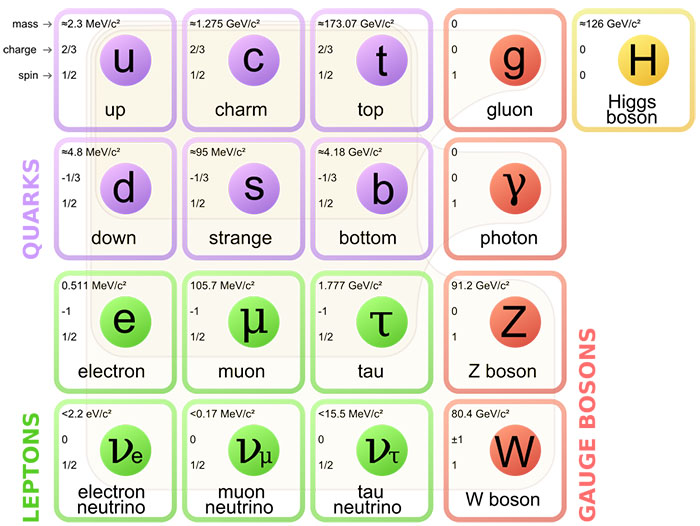
\includegraphics[scale = 0.4]{StandardModel.jpg}
    \caption{The particles of the Standard Model, grouped based on their quantum spin into gauge bosons and fermions (particles that make up all matter).The fermions are further divided into quarks and leptons which are fundamental, and can partake in various interactions that are mediated by the gauge bosons corresponding to each of the three fundamental forces described by the model. The Higgs boson is also included, and is responsible for all of the particles acquiring their mass. Image sourced from \cite{SM_Picture}}
    \label{StandardModel}
\end{figure}
Despite providing a comprehensive description of the fundamental components of nature and the force acting between these, the Standard Model is subject to numerous limitations, the most prominent of which is its inability to account for the gravitational force \cite{Holstein:2006bh}. Furthermore, the nature of dark matter and dark energy, which account for
a large proportion of the matter in the Universe, is not fully understood, and remains an area of ongoing research. A more subtle limitation, however, pertains to a phenomenon known as CP violation and the absence of experimental evidence of this in the strong force, despite being theoretically permissible by the quantum field theory of this force,
known as quantum chromodynamics (QCD) \cite{Garcia_Irastorza_2022}. This is known as the Strong CP problem and forms the basis for motivating particles such as the axion, as well as Axion-Like Particles (ALPs), both of which are described in further detail in the sections that follow.
\section{CP Violation}
The principle of symmetry (i.e. the invariance of a physical system under a transformation) is significant in the study of particle physics. Two symmetries that are of particular interest are those of charge conjugation, denoted $C$, and parity, denoted $P$. Charge conjugation is a transformation wherein particles within a physical system are interchanged with
their antiparticles, as demonstrated in Figure \ref{ChargeConjugation}, while parity refers to the inversion of spatial coordinates of a physical system, as illustrated in Figure \ref{ParityTransformation} below. 
\\
\\
The combination of the abovementioned transformations is referred to as $CP$, and its violation is of particular interest as it provides a possible explanation for the abundance of matter over antimatter in the Universe. CP symmetry has been observed to be preserved in electromagnetic interactions, whilst being violated in weak interactions, as demonstrated by 
a study of the decay of neutral kaons by Cronin and Fitch in 1964 \cite{PhysRevLett.13.138}. While the theory of QCD permits the violation of this symmetry in the strong force, there is no experimental evidence of processes that violate this symmetry. This is referred to as the Strong CP problem, and is essential for the theoretical motivation behind axions and ALPs \cite{PhysRevLett.40.223}.
\begin{figure}[H]
    \centering
    \begin{subfigure}{0.5\textwidth}
        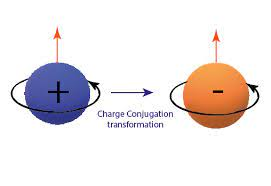
\includegraphics[]{ChargeConjugation.jpg}
        \caption{The charge conjugation transformation $C$, which interchanges particles in a physical system with their corresponding antiparticles. Sourced from \cite{ChargeConj}}
        \label{ChargeConjugation}
    \end{subfigure}
    \hfill
    \begin{subfigure}{0.7\textwidth}
        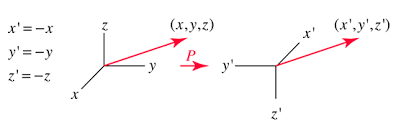
\includegraphics[]{ParityTransformation.png}
        \caption{An illustration of the parity transformation $P$, corresponding
        to the inversion of spatial coordinates in a physical system. Sourced from \cite{ParityTransf}}
        \label{ParityTransformation}
    \end{subfigure}
    \hfill
\end{figure}
\subsection{The Strong CP Problem}\label{StrongCPProb}
The theoretically permissible nature of CP violation in the strong force is evident within the QCD Lagrangian, which can be written in the following form \cite{Michael:920}:
\begin{equation}\label{QCD_Lagrangian}
    \mathcal{L}_{QCD} = -\frac{1}{4}G_{\mu\nu}G^{\mu\nu}-\frac{g_{s}^{2}\theta}{32\pi^{2}}G_{\mu\nu}\tilde{G}^{\mu\nu}+\bar{\psi}(i\gamma^{\mu}D_{\mu}-me^{i\theta'\gamma_{5}})\psi
\end{equation}
where $G_{\mu\nu}G^{\mu\nu}$ represents the gluonic field strength tensor, which is the QCD equivalent of the electromagnetic field strength tensor, $F_{\mu\nu}F^{\mu\nu}$, and $\tilde{G}^{\mu\nu}$ is its dual. By inspection, it is evident that the terms $\theta$ and $\theta'$ in Equation \ref{QCD_Lagrangian} are CP-violating, as they both 
change sign under a parity transformation. The effects of these terms, which can be interpreted as physical angles, are not experimentally observed, thereby suggesting that these angular terms are infinitessimal in magnitude. The angular terms $\theta$ and $\theta'$ can be combined to form a total effective angle, labelled $\bar{\theta}$. The absence
of CP violation in the strong force suggests that $|\bar{\theta}|\approx 0$. This is supported by the experimental measurement of the electric dipole moment (EDM) of the neutron, which impose the constraint $|\bar{\theta}| < 10^{-10}$ \cite{PhysRevLett.124.081803}. This is referred to as a fine-tuning problem, wherein the value of $|\bar{\theta}|$ is constrained to be as small as possible
through the tuning of other parameters in order to maintain consistency with experimental observations \cite{https://doi.org/10.48550/arxiv.hep-ph/9704427}.\\
\\
A more elegant solution to the Strong CP problem was proposed by Peccei and Quinn in 1977 \cite{article}. This solution involved promoting $\bar{\theta}$ to a dynamic field, thereby introducing a spatial and temporal dependence, along with an associated
potential. This field is postulated to have an associated global symmetry, known as the Peccei-Quinn (PQ) symmetry. Spontaneous breaking of this symmetry mandates that $|\bar{\theta}| = 0$, thereby resolving the Strong CP Problem without the need of fine-tuning. This solution 
results in the introduction of the axion, which in turn leads to the motivation of Axion-Like Particles (ALPs) through the similar mechanism of spontaneous symmetry breaking, which is elaborated upon in \cite{Beekman_2019}.
\section{Axions}
Spontaneous breaking of the PQ symmetry described in Section \ref{StrongCPProb} mandates the introduction of a light, pseudoscalar (spin-0 and odd parity) particle known as the QCD axion \cite{article}. Axions obey a well-defined relation between their mass and coupling
to Standard Model particles. For instance, the coupling constant $f_{A}$ of the axion-photon coupling in one of the many axion models is inversely proportional to the mass of the axion, $m_{A}$, as demonstrated in the relationship represented in Equation \ref{AxionMassCoupling} below \cite{Michael:920}:
\begin{equation}\label{AxionMassCoupling}
    f_{A}m_{A} = f_{\pi^{0}}m_{\pi^{0}}
\end{equation}
where $f_{\pi^{0}} = 92$ GeV and $m_{\pi^{0}} = 135$ MeV correspond to the mass and coupling strength to photons of the neutral pion, $\pi^{0}$, respectively.\\
\\
Axions are referred to as pseudo Nambu-Goldstone (pNG) bosons, on account of their zero quantum spin and odd parity. There exist various axion models, which differ in their couplings to fermions and the energy scales involved. A detailed description of two of the most prominent axion models, namely the Kim-Shifman-Vainshtein-Zakharov (KSVZ), and the Dine-Fischler-Srednicki-Zhitnitsky (DFSZ) models can be obtained in \cite{Garcia_Irastorza_2022}.
Despite the variety of axion models that are proposed, these pseudoscalars are known to mix with mesons, and consequently possess a model-independent coupling to photons. This coupling can be expressed through the presence of the following term in the Lagrangian \cite{Garcia_Irastorza_2022}
\begin{equation}\label{AxionPhoton}
    \mathcal{L}_{a_{0}\gamma} = -\frac{g_{a_{0}\gamma}}{4}a_{0}F_{\mu\nu}\tilde{F}^{\mu\nu} = g_{a_{0}\gamma}a_{0}\vb*{E}\cdot\vb*{B}
\end{equation}
where $g_{a_{0}\gamma}$ is the axion-photon coupling, and $F_{\mu\nu}$ and $\tilde{F}^{\mu\nu}$ represent the electromagnetic field strength tensor and its dual respectively. The term on the far right of Equation \ref{AxionPhoton} is an equivalent form of the interaction that is written in terms of the electric and magnetic fields, $\vb*{E}$ and $\vb*{B}$ respectively \cite{Garcia_Irastorza_2022}. Other couplings of axions
to fermions that are of interest for the purposes of detection include those to nucleons and electrons, the latter of which is model-dependent. The phenomenology of axions described above serves as a motivation for the introduction of other light bosons as a consequence of other spontaneously broken symmetries at a higher energy scale $f_{a}$ \cite{Ringwald:2012hr}. These are referred to as axion-like particles, or ALPs
\section{Axion Like Particles (ALPs)}
Spontaneous breaking of other symmetries similar to the Peccei-Quinn symmetry described in Section \ref{StrongCPProb} produces particles similar to the axion, referred to as \textit{axion-like particles} (which will henceforth be referred to as ALPs, or $a_{0}$ in decays). Unlike axions, which are expected to be very light (i.e. within the sub-eV regime), the masses of ALPs 
are not as constrained, thereby implying that these can be arbitrarily heavy. Furthermore, Axion-Like Particles are able to couple to pairs of
gauge bosons (e.g. $\gamma\gamma, gg, HH$) as well as fermions (i.e. leptons and quarks) depending on the model being considered, and are not solely linked to the strong interaction like their
counterparts \cite{Michael:920}. \\
\\
ALPs are of significant importance to advancements in various fields of physics, particularly cosmology. The feeble nature of the interactions between ALPs and Standard Model particles makes them ideal dark matter candidates. In addition to this, they
are believed to be able to offer an explanation of the anomalies in the energy loss of white dwarf stars \cite{Isern_2008}. Their existence can also offer an explanation of the observational hints on extra dark radiation in the primordial plasma during big bang nucleosynthesis in the form
of Cosmic ALP Background (CAB) radiation \cite{https://doi.org/10.48550/arxiv.1407.0546}. Thus, a multitude of experimental methods and strategies have been employed to search for these particles, the most prominent of which include haloscope searches, Light-Shining-Through Wall (LSW) searches, and helioscope searches. These
techniques, along with the constraints that they have imposed on the masses and couplings of ALPs to Standard Model particles are summarised in the sections that follow. The general search strategy and constraints imposed by collider experiments are also summarised in these sections. This, with an enhanced focus on the Large Hadron Collider beauty (LHCb) experiment,
will be the primary emphasis of the remainder of this work. 
\section{Experimental Searches for Axions and ALPs}\label{ALPExpt} 
Since light pseudoscalars are theorised to naturally couple to photons, due to spin-selection rules and mass constraints, the searches for ALPs performed through cosmological and astrophysical observations, as well as those
being conducted at low-energy accelerators exploit the (inverse) Primakoff effect, wherein axions are converted to photons (and vice versa) in collisions with photons, or identically with electromagnetic fields \cite{d'Enterria:2753504}. This is the case with the experimental search strategies
that are summarised below, namely the Light Shining through Walls (LSW) experiments, helioscope, and haloscope searches. Further details on the nature and structure of the search techniques described below can be obtained in \cite{doi:10.1146/annurev-nucl-102014-022120}
\begin{figure}[H]
    \centering      
    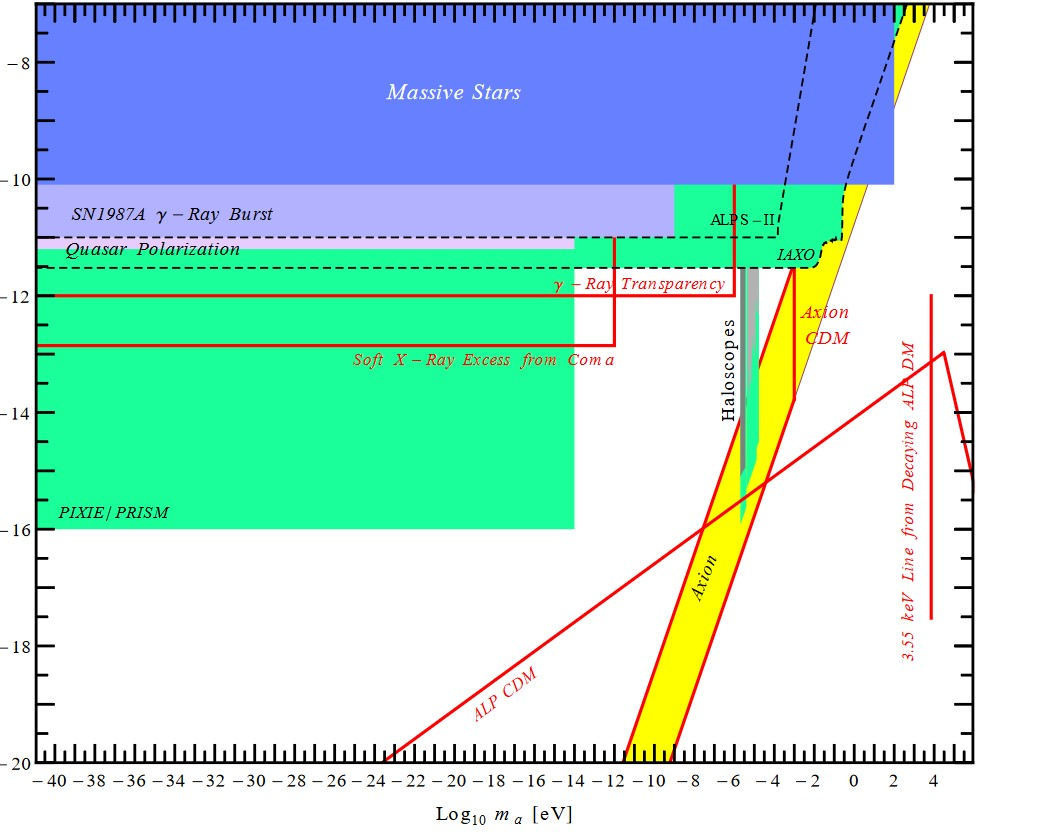
\includegraphics[scale = 0.45]{ALPExperimentalConstraints.jpg}
    \caption{Plot displaying the constraints imposed on the masses and coupling strengths of ALPs to photons by a variety of experiments, such as LSW, helioscope, and haloscope searches (such as ALPS-II and ADMX respectively). Of particular interest are the constraints imposed by the LSW experiments ALPS-II, as well as the helioscope limits expected to be set by IAXO. The bright yellow band indicates
    the prediction for the axion. Figure sourced from \cite{https://doi.org/10.48550/arxiv.1407.0546}}
    \label{ALPExperimentalConstraints}
\end{figure}
\subsection{Light Shining Through Walls (LSW) Searches}
LSW experiments are intended to produce and detect ALPs in the laboratory by sending laser photons along a strong magnetic field,
thereby allowing for their conversion into ALPs towards a blocking wall, behind which these might reconvert into photons, once again in the presence of 
a strong magnetic field \cite{https://doi.org/10.48550/arxiv.1407.0546}. These photons are susceptible to detection. Currently, the best sensitivity of LSW experiments has been establishedd by the Any Light Particle Search
(ALPS I) experiment located at DESY. A successor experiment, known as ALPS II, has also been designed with a high-power laser system, and stronger magnets. The experiment intends to 
probe the ALP parameter space that is favoured by astrophysical observations. However, the ability of LSW experiments to probe other spectral ranges, particularly in the microwave and
X-ray ranges are still in the early stages of development, and are unlikely to yield significant results in the forseeable future \cite{https://doi.org/10.48550/arxiv.1407.0546}.
\subsection{Haloscope Searches}
Haloscopes directly search for galactic halo dark matter axions and ALPs in the laboratory. The most sensitive of these experiments aim to detect the electromagnetic power which is generated from the conversion of dark matter axions and ALPs into detectable photons.
The optimal sensitivity is achieved on resonance, at which point the power output is proportional to the quality factor of the cavity. One experiment that has attained a sensitivity to probe axion dark matter is the Axion Dark Matter Experiment (ADMX). The constraints on the masses
and couplings of ALPs to photons set by this
experiment are indicated by the vertical green band labelled 'Haloscopes' in Figure \ref{ALPExperimentalConstraints} above. The figure also indicates the constraints on the same parameters set by other haloscope experiments such as those performed at the PIXIE and PRISM CMB observatories \cite{https://doi.org/10.48550/arxiv.1407.0546}. Experiments with
higher sensitivities than the ADMX, named ADMX (HF) and ADMX-II, which constitutes an upgrade to the existing ADMX experiment, are also proposed in order to further probe the green regions in Figure \ref{ALPExperimentalConstraints} above. Further information on the status of these experiments, including details of their design and structure are detailed in \cite{ADMX:2020ote} and \cite{Nitta:2022jez}.There is also scope to probe other mass ranges through the recycling of available microwave cavities and magnets at accelerator laboratories \cite{https://doi.org/10.48550/arxiv.1407.0546}
\subsection{Helioscope Searches}
Helioscopes are designed to detect solar ALPs (i.e. the ALPs that are produced in the Sun). The detection occurs through the conversion of the ALPs into photons, which is facilitated by a strong magnet that is directed at the Sun.
Presently, an helioscope named the International Axion Observatory (IAXO), which has been modelled largely based on its predecessor, the CERN Axion Solar Telescope (CAST), with enhancements made to the design in the form of a superconducting
toroidal magnet and a larger aperture, as well as a detection system consisting of large X-ray telescopes coupled to ultra-low background X-ray detectors, and a large, robust tracking system. These are intended to probe the regions labelled 'IAXO'
in Figure \ref{ALPExperimentalConstraints} above. Further details on the design and operation of the IAXO experiment, including details pertaining to a smaller scale experiment known as the BabyIAXO, can be found in \cite{MargalejoBlasco:2022ncg}.
\subsection{Collider Searches}   
As a consequence of the (inverse) Primakoff effect, described in further detail in \cite{Primakoff:1951iae}, the ALP searches conducted at colliders aim to exploit the coupling of these particles to photons by examining decays which contain photons either
in their initial or final states \cite{d'Enterria:2753504}. This permits for a link to be established with the various other search strategies described above. Furthermore, the identification of these decays over intrinsically large hadronic backgrounds becomes
simpler, thereby suggesting that collider searches provide a strong prospect for probing different regions in the $(m_{a}, g_{a\gamma})$ parameter space to those containing the limits set by other search methods \cite{d'Enterria:2753504}.\\
\\
Recently, collider experiments have aimed to focus their attention on ALP masses above the MeV scale. The decay rate of $a_{0}\rightarrow\gamma\gamma$ is dependent on the third power of the ALP mass, the decay rate 
diminishes such that the ALP leaves the detector and appears as an invisible particle as its mass increases. There also exist fixed-target proton and electron experiments wherein photons are produced by meson decays or bremsstrahlung
respectively. The photons that are present in the final state of each of these processes can convert into ALPs via the Primakoff process off a nuclear target. The inverse Primakoff process is exploited when the decay mode $a_{0}\rightarrow\gamma\gamma$ is probed for the presence of ALPs. Various collider experiments have
aimed to constrain the masses and couplings of ALPs to photons through a multitude of decay modes, the most prominent of these being CLEO and BaBar, where mono-photon final states with missing energies from long-lived "invisible" ALPs with via radiative decays are investigated, as well as diphoton and triphoton final states, as 
examined by the LEP-I and LEP-II experiments via, for instance, the decay mode $e^{+}e^{-}\rightarrow\gamma a_{0}$ (where $a_{0}\rightarrow\gamma\gamma$). Each of the experiments described above probes a different region in the $(m_a, g_{a\gamma})$ parameter space. The constraints imposed on these parameters is summarised in Figure
\ref{ALPColliderConstraints} below. Figure \ref{ALPExperimentalAndColliderConstraints} provides a more holistic perspective on the collider constraints by also including the regions of the parameter space that have been probed by the multitude of experimental techniques described above. The regions probed by the ATLAS and CMS detectors, which are
sub-experiments of the Large Hadron Collider (LHC) are of particular interest, as they investigate the phenomenon in lead-lead (Pb-Pb) collisions, in contrast to the proton-proton (pp) collisions performed at the LHCb \cite{d'Enterria:2753504}
\begin{figure}[H]
    \begin{subfigure}{0.5\textwidth}
    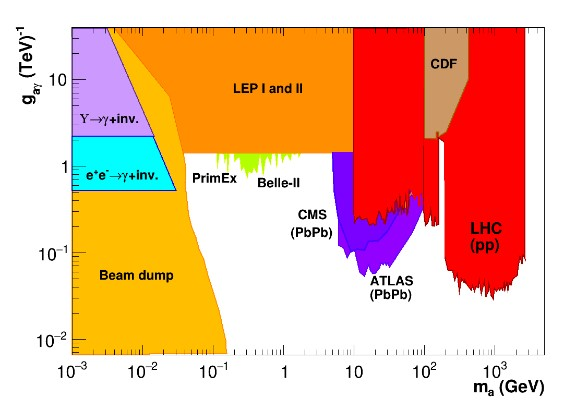
\includegraphics[scale = 0.7]{ALPColliderConstraints.jpg}
    \caption{Detailed bounds on the $(m_{a}, g_{a\gamma})$ parameter space by ALP searches from existing collider and accelerator experiments.}
    \label{ALPColliderConstraints}
    \end{subfigure}
    \hfill
    \begin{subfigure}{0.4\textwidth}
        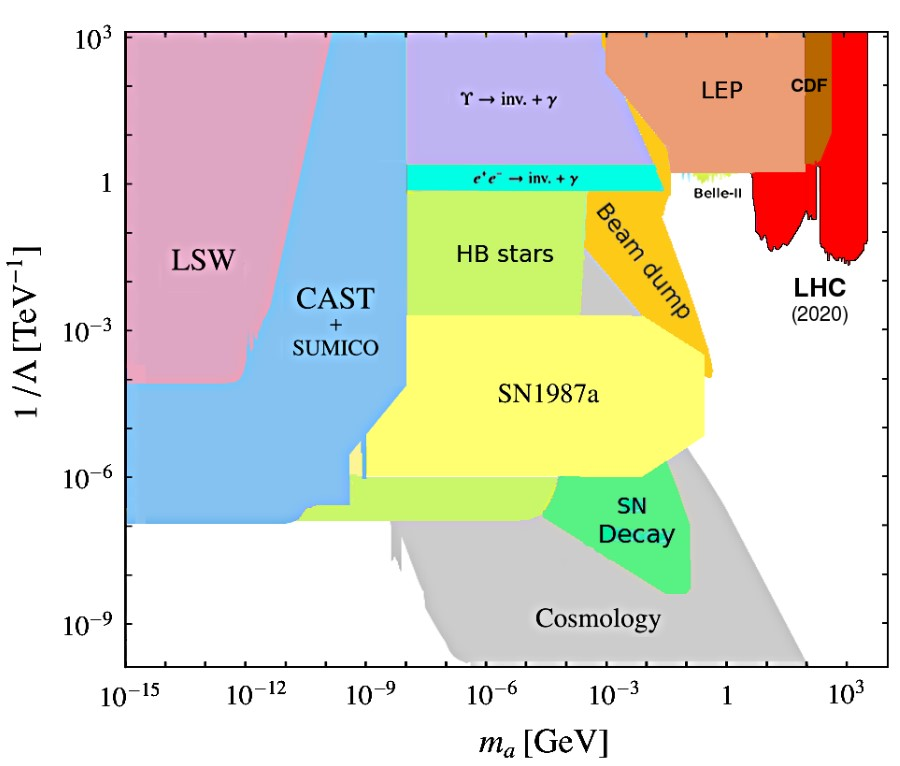
\includegraphics[scale = 0.35]{ALPExperimentalAndColliderConstraints.jpg}
        \caption{Limits on $(m_{a},g_{a\gamma})$ imposed by the techniques described in Section \ref{ALPExpt}. The collider constraints in Figure \ref{ALPColliderConstraints} are also evident on the far right of this figure.}
        \label{ALPExperimentalAndColliderConstraints}
    \end{subfigure}
    \hfill
\end{figure}
\section{The $B^{0}\rightarrow K^{*}a_{0}, a_{0}\rightarrow\gamma\gamma$ Decay Process} 
\begin{figure}[H]
    \centering
    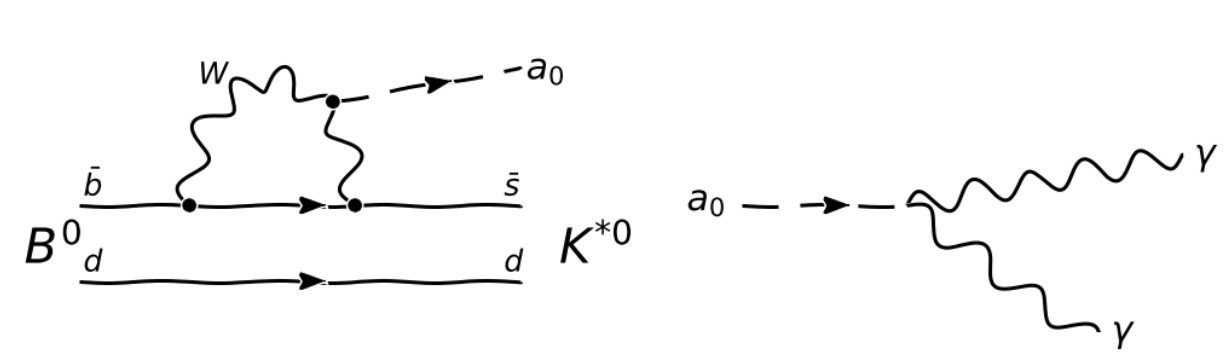
\includegraphics[scale=0.45]{FCNCALP.jpg}
    \caption{Left- One-loop level Feynman diagram of the Flavour Changing Neutral Current (FCNC) process which is responsible for the $b(\bar{b})\rightarrow s(\bar{s})$ quark transition in the decay process described by the relation (\ref{DecayChannel}). This interaction takes place through the exchange of a charged $W$ boson, and is forbidden at tree-level in the Standard Model. Figure adapted from \cite{Izaguirre2016ANF}. Right- Visual representation of the $a_{0}\rightarrow\gamma\gamma$ decay, adapted from \cite{Michael:920}}
\end{figure}
The model considered in the sections that follow is described in detail in \cite{Izaguirre2016ANF}. The model describes a
coupling to the weak gauge bosons $W^{\pm}$, which gives rise to observable signatures within the detector apparatus. This model has a
zero coupling with gluons, and its effective Lagrangian is given by
\begin{equation}
    \mathcal{L} = (\partial_{\mu}a)^{2}-\frac{1}{2}m_{a}^{2}a^{2}-\frac{g_{aW}}{4}W_{\mu\nu}\tilde{W}^{\mu\nu}
\end{equation}
where $g_{aW}$ is the coupling between the ALP field $a$ and the electroweak gauge boson field $W$. Furthermore, $\tilde{W}^{\mu\nu} = \epsilon^{\mu\nu\alpha\beta}W_{\alpha\beta}/2$ \cite{Izaguirre2016ANF}.Promising decay channels which could exhibit this coupling can take
place through a Flavour Changing Neutral Current (FCNC) process, further detailed in \cite{Archilli:2017xmu}. One such decay channel is 
\begin{equation}\label{DecayChannel}
    B^{0}\rightarrow K^{*}a_{0}, a_{0}\rightarrow\gamma\gamma
\end{equation}

The above decay channel is of interest, as the decaying particle is a neutral $B$ meson, which has been studied extensively by a multitude of accelerators and colliders that are optimised to generate and detect
them. Figure  The Large Hadron Collider beauty (LHCb) is one such detector that possesses a substantial amount of data pertaining to the decay of $B$-mesons. For this reason, the search for ALPs that are produced by the decay channel
described in (\ref{DecayChannel}) appears to be viable and worth pursuing at the LHCb. The design, structure, and computational framework of the experiment are further detailed in the subsequent chapters






\chapter{The LHCb Detector}
\section{Structure of the LHCb Detector}
The Large Hadron Collider beauty (LHCb) detector is a single-arm spectrometer possessing a forward angular coverage from
approximately 10 mrad to 300 (250) mrad in the bending (non-bending) plane \cite{https://doi.org/10.48550/arxiv.0910.1740}
The structure of the detector is motivated by the fact that both the $b$ and the $\bar{b}$ hadrons are predominantly produced in the
same forward or backward cone. The components that enable the identification of particles, and aid the deduction of their properties include
the vertex locator system (VELO), the tracking system, comprising of a Trigger Tracker (a silicon microstrip detector, TT) located in front 
of the magnet, three tracking stations behind the magnet made up of silicon microstrips in the inner and outer parts (labelled IT and OT respectively),
two Ring Imaging Cherenkov counters (labelled RICH1 and RICH2 respectively), as well as a calorimeter system, comprising of a Scintillating Pad Detector and Preshower
(SPD/PS) and electromagnetic and hadronic calorimeters (ECAL and HCAL respectively) \cite{https://doi.org/10.48550/arxiv.0910.1740}. The layout of the LHCb spectrometer including the relative positions of the components described above, is illustrated in Figure \ref{LHCbDetector}.\\
\\
Of the abovementioned components, the dipole magnet, VELO, and ECAL play a significant role
in the analysis of the decay described in Section \ref{DecayProcess}. The structure of these sections of the
detector is further elaborated on in the sections that follow.
\begin{figure}[H]
    \centering
    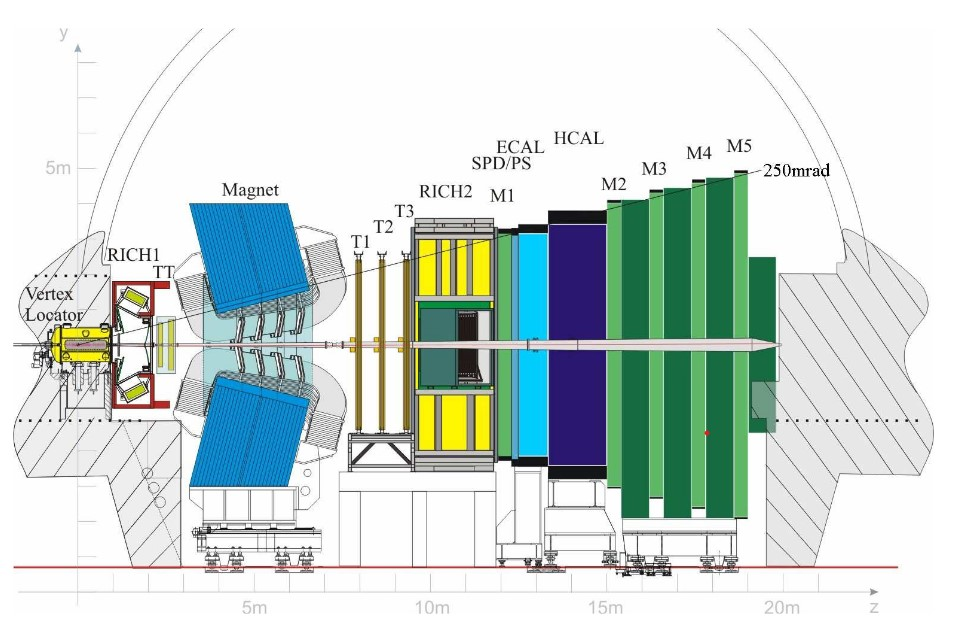
\includegraphics[scale = 0.45]{LHCbDetector.jpg}
    \caption{Diagram of the LHCb detector illustrating its various components. The coordinate system is oriented such that the beam is directed along the $z$ axis, and the $y$ axis is oriented along the vertical. Figure sourced from \cite{AbellanBeteta:2020amj}}
    \label{LHCbDetector}
\end{figure}
\subsection{Vertex Locator (VELO)}\label{VELO}
The Vertex Locator (VELO) is a silicon-tracking detector in the spectrometer, positioned around the proton-proton interaction region of the LHCb experiment shown in Figure (\ref{LHCbDetector}) above, and is responsible for the high-precision reconstruction of the primary and secondary vertices, and impact parameters of particle decays. In addition to this, it is a key
contributor to the measurements of particle lifetimes \cite{Kopciewicz_2022}.It was designed to optimise the angular coverage, triggering, reconstruction efficiency, and decay time of the resulting particles \cite{Aaij_2014}. The measurements made by the VELO are a vital input to the second level trigger (L1), which enhances the b-quark decay content of the data.\\
\\
The detector comprises of a series of silicon-stations that are aligned with the beam direction. These are placed at a radial distance from the beam. These detectors are subjected to a substantial amount of radiation, due to their proximity to the LHC beam
\subsection{Ring Imaging Cherenkov (RICH) Detector}
The Ring Imaging Cherenkov (RICH) system at the LHCb consists of two detectors, namely RICH1 and RICH2, and is responsible for the identification of charged hadrons (such as $\pi, K$ and $p$). RICH1 is placed as close as possible to the interaction region, and is located immediately downstream of the VELO, described in Section \ref{VELO} above. This detector is intended to cover the low and intermediate momentum region (ranging from 2 to 40 GeV/c) over the full spectrometer angular acceptance of 25-300 mrad \cite{Adinolfi_2013}. RICH2, on the other hand, is placed downstream of the magnet, as it is intended to
identify particles possessing higher momenta (i.e. between 15-100 GeV/c) over the angular range 15-120 mrad, which are less affected by the magnetic field \cite{Adinolfi_2013}.\\
\\
RICH1 contains aerogel and two fluorobutane (C$_{4}$F$_{10}$) gas radiators which provide Particle Identification (PID) for positive kaons above 2 GeV/c and $\pi$-$K$ separation of up to 10 GeV/c.  within the acceptance. The detector consists of an optical system possessing spherical mirrors located in the LHCb acceptance that are traversed by charged particles and photons. The structure and materials used to construct these mirrors are elaborated upon in \cite{Antunes-Nobrega:630827}. The Cherenkov light emitted by particles as they traverse the detector is focused onto photon detector planes by these spherical mirrors, which are tilted, as well as secondary plane mirrors \cite{Antunes-Nobrega:630827}.Figure 
\ref{RICH1Layout} below illustrates the layout of the RICH1 detector, with the $z$ axis oriented to run horizontally. 
Further details on the structure and performance of RICH1 can be obtained in \cite{Adinolfi_2013} and \cite{Antunes-Nobrega:630827}. 
\begin{figure}[H]
    \centering
    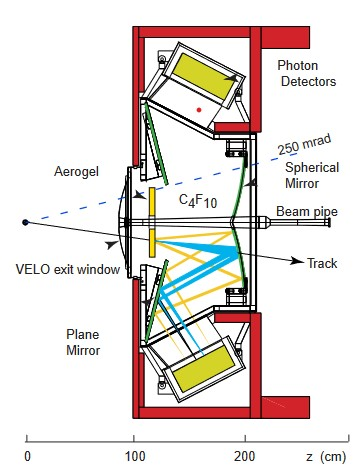
\includegraphics[scale=0.8]{RICH1Layout.jpg}
    \caption{ADD CAPTION}
    \label{RICH1Layout}
\end{figure}
The optical arrangement of the RICH2 detector is symmetric about the vertical plane. Much like RICH1, the detector possesses two sets of spherical and plane mirrors that focus Cherenkov radiationonto two photon detector arrays. CF$_{4}$ is used as the radiator material \cite{Harnew:2008zz}. Figure \ref{RICH2Layout} represents a schematic of the RICH2 detector.
\begin{figure}[H]
    \centering
    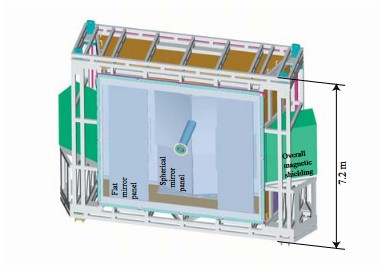
\includegraphics{RICH2Layout.jpg}
    \caption{ADD CAPTION}
    \label{RICH2Layout}
\end{figure}
\subsection{Magnet} 
A warm dipole magnet is employed within the design of the LHCb in order to measure the momenta of charged particles. This measurement 
encompasses the forward acceptance of $\pm$ 250 mrad vertically and of $\pm$ 300 mrad horizontally
\subsection{Electromagnetic Calorimeter (ECAL)}
The ECAL aims to provide the precision measurement of photons in order to enable the reconstruction of $B$-decay modes containing either a photon or $\pi^{0}$ \cite{GOLUTVIN2003258}.
The calorimeter is constructed in a "shashlik" structure, comprising of three segmented sections, each comprising modules of an identical square size of 121.2 mm, but with varying numbers of
readout cells. This 'shashlik' structure had been chosen so as to enhance the energy resolution, response time, and the reliability of the calorimeter in an environment that is prone to radiation, in a cost effective manner \cite{Amato:494264}. Each module (depicted in Figure \ref{ECALModule} below) is comprised of alternating layers of a synthetic material made from polyethelene fibers known as Tyvek, a scintillator tile of thickness 4 mm, and a lead absorber plate of thickness 2 mm.
The system possesses a total of 67 scintillator and 66 absorber layers, combining to a resultant module depth of approximately 25 radiation lengths \cite{AbellanBeteta:2020amj}. The scintillation light is re-emitted and transported along fibres that penetrate the entire
module, and is then read out with a photomultiplier tube \cite{AbellanBeteta:2020amj}.
\begin{figure}[H]
    \begin{subfigure}{0.4\textwidth}
    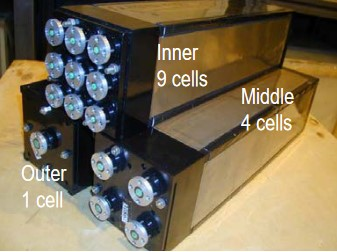
\includegraphics[scale = 0.75]{ECALModule.jpg}
    \caption{ADD CAPTION}
    \label{ECALModule}
    \end{subfigure}
    \hfill
    \begin{subfigure}{0.5\textwidth}
        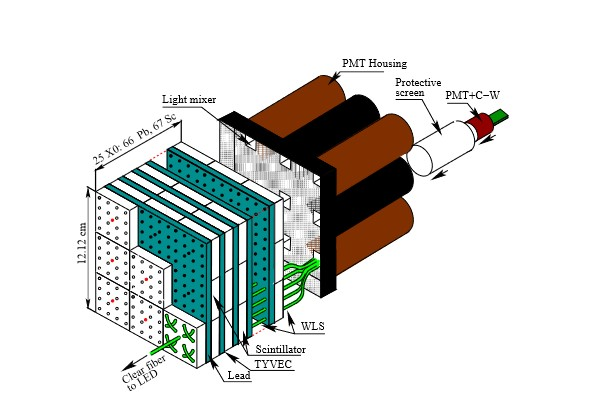
\includegraphics[scale = 0.65]{ECALStructure.jpg}
        \caption{ADD CAPTION}
        \label{ECALStructure}
    \end{subfigure}
    \hfill
\end{figure}
The energy resolution, $\frac{\sigma_{E}}{E}$, (i.e.the accuracy of the detector in determining the energy of the incoming radiation) of the outer module of the ECAL, which consists of one cell (depicted in Figures \ref{ECALModule} and \ref{ECALStructure} respectively) has been measured to be \cite{GOLUTVIN2003258}:
\begin{equation}
    \frac{\sigma_{E}}{E} = \frac{9.4\%}{\sqrt{E}}\oplus 0.8\%
\end{equation}
The ECAL is a key component of the search for ALPs at the LHCb experiment, since it measures the transverse energy $E_{T}$ of the photons in the decay channel of interest (see Section \ref{DecayChannel}), is a vital measurement for this analysis. Further details on the structure and performance of the ECAL can be obtained in Refs \cite{Amato:494264}, \cite{AbellanBeteta:2020amj}, and \cite{GOLUTVIN2003258}.
\section{Data Analysis at the LHCb}
The Large Hadron Collider provides proton-proton collisions to the LHCb approximately 40 million times per second, thereby generating a significant amount of data. In order to retain the data from events that are deemed to be of interest for analyses, the plethora of data must be filtered efficiently, and the algorithms
implemented must be sufficiently intricate, so as to be able to manage the complexity of the data being processed. The LHCb experiment implements a data flow which enables the aforementioned objectives to be addressed. The flow of data through the LHCb system is further detailed in the sections that follow.
\subsection{The LHCb Data Flow}\label{LHCbDataFlow}
The collision events recorded by the LHCb detector proceed through various steps, each of which is controlled by an application that processes the data in a way that maximises the efficiency of data acquisition and also enhances the quality of the obtained. The data from the detector is first filtered through hardware and software components, known as the L0 trigger, and the high level trigger (HLT) respectively. Following this, the data is
reconstructed to transform the detector into objects such as tracks and clusters, which are stored in an output file in a 'DST' format. Data from this files is further filtered through a set of selections known as the stripping, the output of which is produced in either a DST or a '$\mu$DST' (micro-DST) format.\\
\\
A substantial amount of Monte Carlo (MC) simulated data is also generated in parallel to the detector data as part of the data flow. This is processed in a very similar manner to the detector data outlined above. Figure \ref{LHCbData} illustrates the abovementioned stages of the data flow and processing. The framework implemented to generate and process the simulated events described above, along with its constituent components are further elaborated upon in the subsequent sections
\begin{figure}[H]
    \centering
    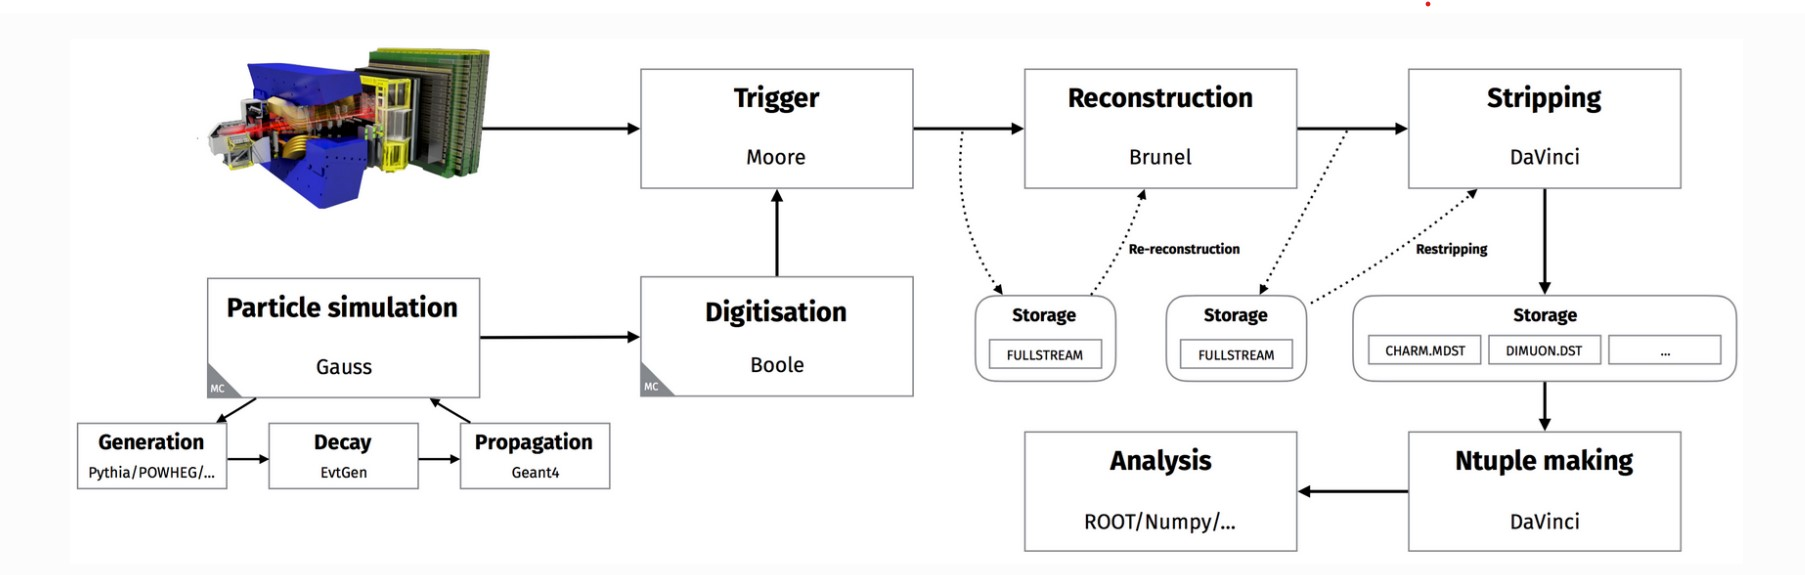
\includegraphics[scale = 0.4]{LHCbDataFlow.jpg}
    \caption{LHCb Data Flow}
    \label{LHCbData}
\end{figure}
\subsection{The LHCb Simulation Framework}
The MC simulated data that is processed in parallel to the detector data flows through a similar pipeline to its counterpart, with necessary steps in place to mimic the proton-proton collisions and the detector response. The former, and the subsequent hadronisation and decay of the resultant particles 
are controlled by the Gauss application, which is responsible for calling the various compatible Monte Carlo generators such as Pythia and POWHEG, as well as to control applications such as EvtGen and Geant4, which describe the decays of simulated particles and simulate their traversal through and interaction with
the detector. On the other hand, the latter entails the transformation of the simulated hits made in the virtual detector into signals that mimic the real detector. This process is regulated by the Boole application, whose output is designed to closely match that of the real detector, such that the simulated data produced can be 
processed via the process described in Section \ref{LHCbDataFlow} above. 
\subsubsection{Gauss}
Gauss is a component of the simulation that intends to mimic the working of the spectrometer to enable the understanding of the experimental conditions and its performance \cite{Tlustos:913827}.
It comprises of two independent phases that are integrated and are typically run as a single job, but can be run separately if necessary. The first phase consists of the event generation
of proton-proton collisions and the decaying of the B mesons into channels of interest. This tool is interfaced to Pythia for the event production, and to a specialised decay package known as
EvtGen (see Section \ref{EvtGen} below). This phase also allows for the interfacing of other event generator engines if necessary. The particles produced are stored in the HepMC \cite{BUCKLEY2021107310} generic format that can be made persistent if the 
phase is run independently (i.e. in \textit{stand-alone} mode).\\
\\
The second phase consists of the tracking of the particles produced in the proton-prpton interactions within the detector. The physics processes undergone by the particles as they traverse the experimental setup are
regulated by the Geant4 toolkit (see Section \ref{Geant4} below), which interacts with Gauss using a host of interfaces and converters which enable the conversion of the LHCb detector geometry into the Geant4 geometry. In addition to this, it converts the output of the first phase of Gauss described above, to the Geant4 input format.\\
\\
Figure \ref{GaussSoftwareStructure} is a visual representation of the structure of the Gauss software that has been described above, while Figure \ref{GaussDependenices} depicts the various dependencies upon which the software has been built. These are further elaborated upon in the sections that follow. Further information on the architecture of the
Gauss software can also be obtained in \cite{Tlustos:913827} and \cite{Belyaev_2011}.
\begin{figure}[H]
    \begin{subfigure}{0.4\textwidth}
    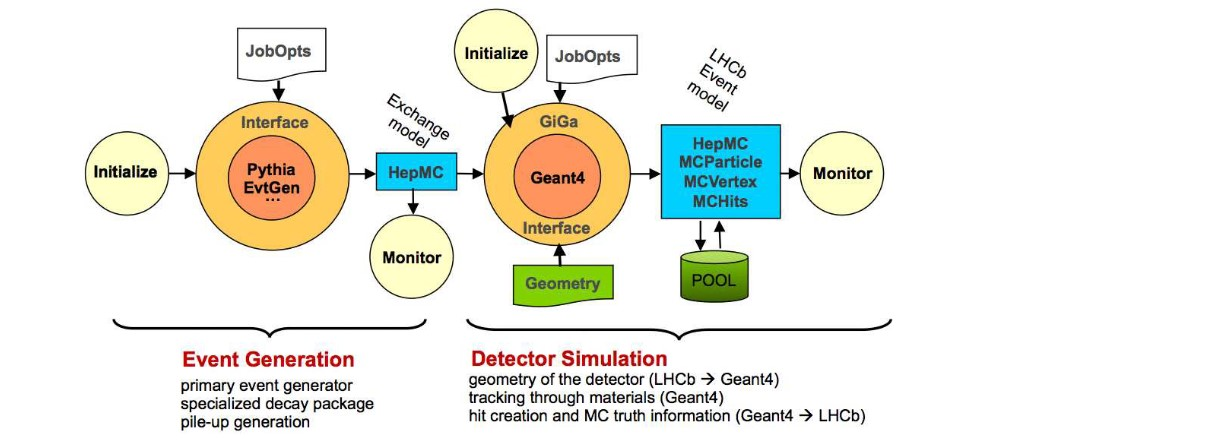
\includegraphics[scale = 0.5]{GaussSoftwareStructure.jpg}
    \caption{ADD CAPTION}
    \label{GaussSoftwareStructure}
    \end{subfigure}
    \hfill
    \begin{subfigure}{0.4\textwidth}
        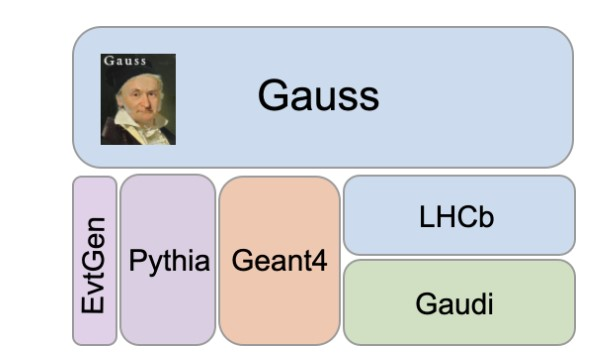
\includegraphics[scale = 0.55]{GaussDependenices.jpg}
        \caption{ADD CAPTION}
        \label{GaussDependenices}
    \end{subfigure}
    \hfill
\end{figure}
\subsubsection{EvtGen}\label{EvtGen}
The EvtGen package is an event generator that is designed for the simulation of the physics of $B$-decays. The package provides a framework to handle complex sequential and CP violating decays. The simulation of these decays proceeds
using decay amplitudes, rather than probabilities. The amplitude for each node in a decay is used to simulate the entire decay chain, including all angular and time dependent correlations \cite{LANGE2001152}. The implementation of each decay amplitude is independent
of how the parent particle was produced, or how the daughter particles are to decay. The package implements an algorithmm that simulates correlations given individual decay amplitudes, which involves summing over the spin degrees of freedom of the daughters of the B-meson, to perform event selection. A more
detailed overview of this procedure can be obtained in \cite{LANGE2001152}.
\subsubsection{Pythia}
The PYTHIA program is a standard tool for the generation of high-energy collisions \cite{SJOSTRAND2015159}. It constitutes a coherent set of
physics models for the evolution from a few-body hard process to a complex multihadronic final states, and contains numerous libraries of 
hard processes and models for initial and final state parton showers, multiple parton-parton interactions, beam remnants and particle decays. It 
also possesses a set of utilities and interfaces to external programs. The present version of the tool, PYTHIA 8, represents a complete rewrite in the C++ programming language, thereby contrasting
with its predecessors that were implemented in Fortran. The program presently only works with hadron-hadron and lepton-lepton collisions. The outgoing particles are produced in vacuum, and the simulation of the interaction of the produced particles with detector material is \textit{not} included in Pythia, and requires interfaces to external detector simulation codes, which can either be written by the user, or accomplished through the use of the HepMC interface. The hard processes, parton showers, multiple interactions,
beam remnants, and hadronisations that are to culminate in a complete event generator can be crudely divided into three stages, which are as follows:
\begin{itemize}
    \item The generation of a "process" that decides the nature of the event. This would generally be a "hard process" (i.e. $gg\rightarrow h_{0}, Z^{0}Z^{0}\rightarrow \mu^{+}\mu^{-} q\bar{q})$ that is calculated in perturbation theory. Only a small number of particles are defined at this level, merely to cover the key aspects of the event structure
    \item The generation of all subsequent activity at the partonic level, including the initial and final state radiation, multiple parton-parton interactions and the structure beam remnants. Much of this phenomena can be described accurately by perturbation theory, but the aspects that cannot be described in such a way also become important at this stage. Upon conclusion of this step, one can obtain a realistic partonic structure
    \item The hadronisation of the abovementioned parton configuration by string fragmentation, followed by the decays of unstable particles. This part is largely nonperturbative, and therefore requires comprehensive modelling and tuning, or parametrisations of existing data, as is necessary for decays. The conclusion of this stage provides the user access to realistic events
\end{itemize}
Orthogonal to the abovementioned subdivisions, there exists a broader classification wherein the user interaction with the generator occurs in three phases, namely:
\begin{itemize}
    \item Initialisation, where the tasks that are to be performed
    \item Generation of individual events (known as the "event loop")
    \item Finishing, where the final statistics are made available
\end{itemize}
One must note that the subdivisions (and orthogonality of the phases described above) are not rigid, and that multiple utilities and tasks extend across the abovementioned categories
\subsubsection{Geant4}\label{Geant4}
The Geant4 toolkit had been developed as the basis for the simulation framework, and as such, it is intended to have well-defined interfaces to other components, as well as to provide parts that can be used by these components. 
There exist seven key domains of the simulation of the traversal of particles through matter, namely:
\begin{itemize}
    \item Geometry and materials
    \item Particle interactions in matter
    \item Tracking management
    \item Digitisation and hit management
    \item Visualisation and visualisation framework
    \item User interface
\end{itemize}
Each of the domains described above are represented by class categories with coherent interfaces, and a corresponding working group with a well-defined responsibilities. The toolkit offers the user the ability to construct a geometric model 
with numerous components of varying shapes and materials. Furthermore, the user is able to define "sensitive" elements that enable the logging of information that is necessary to simulate detector responses.\\
\\
Geant4 also provides an extensive list of physics processes to model the behaviour of particles, enabling the user to choose between, add to, and modify a variety of implementations and approaches that are provided. In addition to this, the user is able to visualise the geometry
and tracks with a multitude of graphics systems and a user interface, which can be implemented over other systems of the user's choice. The structure of the toolkit can be described as a modular and hierarchical in nature, with dependencies forming links between the different sub-domains,
as illustrated in Figure \ref{Geant4Structure} below. Further detail on the nature of the sub-domains and dependencies depicted in this figure can be obtained in \cite{GEANT4:2002zbu}.
\begin{figure}[H]
    \centering
    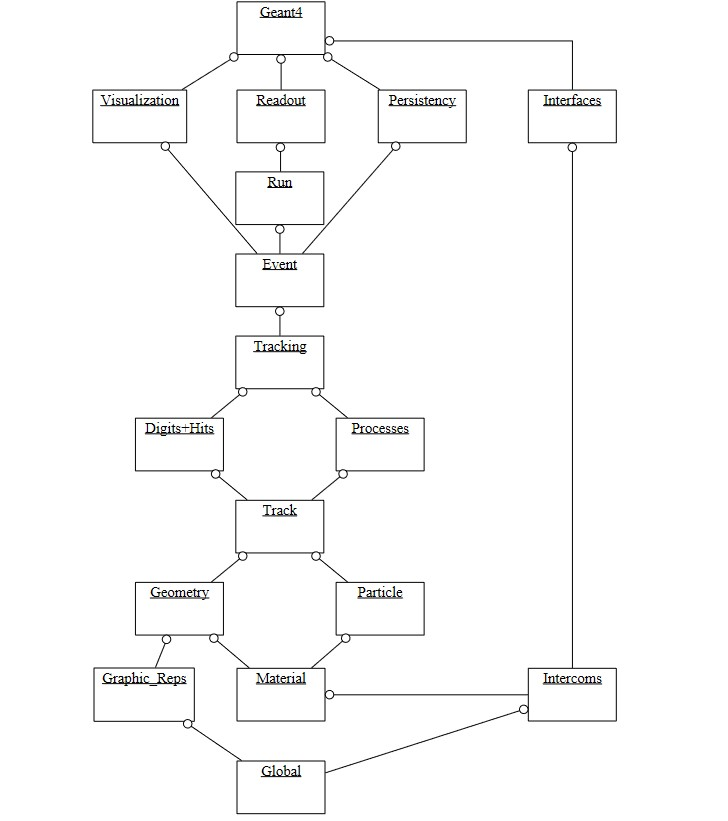
\includegraphics[scale=0.6]{Geant4Structure.jpg}
    \caption{ADD CAPTION}
    \label{Geant4Structure}
\end{figure}
\subsubsection{Gaudi}
The Gaudi software has been developed with the intention of being able to build the large variety of applications necessary for high energy physics experiments, ranging from the simulation of events to the user analysis and the event display. Its design exploits object-oriented methodologies in order to address key criteria pertaining to the separation of data and algorithms, as well as that of persistent and transient data, among other aspects. \\
\\
The Gaudi architecture can broadly classified into three categories as follows \cite{BARRAND200145}:
\begin{itemize}
\item[-] \textbf{Algorithms and Application Manager:} Algorithms are a series of generic interfaces that are the fundamental components of applications that process event data. The application manager sits atop a hierarchy of algorithms, and is responsible for the instantiation and calling of these.
\item[-]\textbf{Transient Data Stores:} The data objects required by the algorithms are organised in various transient data stores, which store event data, which is valid only during the time it takes to process one event. Likewise, detector data, that generally has a lifetime of multiple events, is stored within the transient detector store. There also exists a data store for statistical data, which typically has the lifetime of a complete job, known as a transient histogram and n-tuple store. 
\item[-] \textbf{Services:} Services are a category of components which offer all the services necessary by algorithms (e.g. those for managing the various transient stores, or for managing the conversion between transient and persistent data). Services that facilitate visualisation and event selection also exist within the architecture
\end{itemize}
Figure \ref{GaudiArchitecture} is a depiction of the Gaudi architecture described above.The key components (i.e. the algorithms, application manager, transient data stores, and services), as well as the relationship between these are indicated in this figure. Further detail on the nature of the components described in the diagram can be obtained in \cite{BARRAND200145} and \cite{Clemencic:2010zz}.
\begin{figure}[H]
    \centering 
    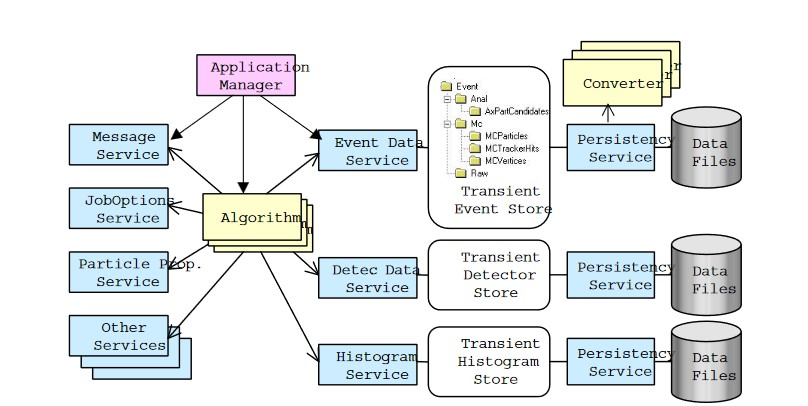
\includegraphics[scale=0.8]{GaudiArchitecture.jpg}
    \caption{ADD CAPTION}
    \label{GaudiArchitecture}
\end{figure}





\chapter{Experimental Methods}
\input{Chapter_3.tex}
\chapter{Results}
\chapter{Discussion}


% Can add more Chapters just follow the same idea above. 
% If you want a different name for the chapter in the header edit the above line as follows \chapter[New Name]{Official Chapter Name}

%##########################################################
\newpage
\chapter*{Conclusion}

% Add Conclusion here

\addcontentsline{toc}{chapter}{Conclusion}
\addcontentsline{toc}{chapter}{References}
%%%%%%%%%%%%%%%%%%%% REFERENCES %%%%%%%%%%%%%%%%%%

% The best way to enter references is to use BibTeX:
%\bibliography{example} % if your bibtex file is called example.bib
\footnotesize
% uncomment and change to the bibiliography style you prefer
%\bibliographystyle{apalike}
%\bibliography{refs}

%%%%%%%%%%%%%%%%% APPENDICES %%%%%%%%%%%%%%%%%%%%%

%\appendix

%\section{Some extra material}

%If you want to present additional material which would interrupt the flow of the main paper,
%it can be placed in an Appendix which appears after the list of references.

%%%%%%%%%%%%%%%%%%%%%%%%%%%%%%%%%%%%%%%%%%%%%%%%%%

% Don't change these lines
%\bsp	% typesetting comment
\label{lastpage}
\end{document}
